\documentclass[9pt]{article}
% \documentclass[10pt,journal]{IEEEtran}
\usepackage{braket}
% Language setting
% Replace `english' with e.g. `spanish' to change the document language
\usepackage[spanish]{babel}
% \usepackage{biblatex}
% %\bibliographystyle{plain}
% \bibliography{sample}
\usepackage{lipsum}
\usepackage{biblatex}
% \addbibresource{bibliografia.bib}
% \bibliography{bibliografia}
\usepackage{physics}
% \usepackage{luacode} % for "\luaexec" macro
% \newcommand\Hats[1]{\luaexec{%
%    tex.sprint (( string.gsub ( "#1" , "\%u", "\\hat{\%0}" )) )}}
% Set page size and margins
% Replace `letterpaper' with `a4paper' for UK/EU standard size
\usepackage[a4paper,top=1.15cm,bottom=2cm,left=1cm,right=1cm,marginparwidth=1.75cm]{geometry}
% Useful packages
\usepackage{sectsty}
\usepackage{float}
\sectionfont{\fontsize{12}{15}\selectfont}
\usepackage{svg}
\usepackage{mathrsfs}
% \usepackage{amsmath}
\usepackage{wrapfig}
\usepackage{graphicx}
\usepackage{sidecap}
\usepackage{xfrac} 
\usepackage[colorlinks=true, allcolors=blue]{hyperref}
\usepackage[T1]{fontenc}
% \usepackage{mathpazo} % cambiar fuente 
\usepackage{cmbright} % cambiar fuente÷ 

\usepackage{booktabs}
\usepackage{caption} 
\usepackage{subcaption}
\captionsetup[table]{skip=3pt}
\usepackage{tabularray}
\usepackage{fancyhdr} % Paquete para encabezados y pies de página
\captionsetup[table]{skip=3pt}
\usepackage{tabularray}
\usepackage{fancyhdr} % Paquete para encabezados y pies de página
\usepackage{array}
\usepackage{amsmath,amssymb}
\usepackage{blindtext}
\usepackage{multicol}
% \usepackage[adjustbox]
%me cago en emma
% \begin{center}
% \includegraphics[width=\linewidth]{grafico.png}
% \captionof{figure}{Este gráfico ocupa solo la columna.}
% \label{fig:ejemplo-col}
% \end{center}

\newcommand{\hamilton}{\mathcal{H}}
% \pagecolor{black}
% \color{white}

\newenvironment{Figure}
  {\par\medskip\noindent\minipage{\linewidth}}
  {\endminipage\par\medskip}



\begin{document}

\begin{center}
    {\Large{Termo IB - Resumen de fórmulas}}
\end{center}

\begin{multicols}{2}

% \section{Series}


\section{Gases ideales}
\begin{equation*}
    PV = nRT \quad P\mathcal{M}  = \rho RT,\quad \text{$\rho\equiv$ densidad, $\mathcal{M}\equiv$ Masa molar}
\end{equation*}

\section{Conservación de la energía}

\begin{gather*}
    dE = dU + \sum dE_{i} = \delta Q - \delta W\\
    dU = nc_vdT \qquad dH = dU + d(PV)\\
    \text{Si P = cte},\quad dH = dU +PdV = nc_pdT
\end{gather*}

\section{Transformaciones adiabáticas cuasiestáticas en gases}
\begin{gather*}
    c_V = \{\sfrac{3}{2}R,\sfrac{5}{2}R,3R\} \quad c_P = c_V + R\\
    \gamma = \frac{c_P}{c_V} \quad Tv^{\gamma-1}=c_1; TP^{(1-\gamma)/\gamma}=c_2; Pv^\gamma=c_3;\\
    c_P=\frac{\gamma}{\gamma-1}R \qquad c_V = \frac{1}{\gamma-1}R
\end{gather*}

\section{Sistemas abiertos}
\begin{gather*}
    h^0 = h+gz +\frac{1}{2}c^2\\
    dE_{VC} = \delta Q + \sum_{k}h_{in}^0\left|\delta m\right| - \sum_{k}h_{out}^0\left|\delta m\right| - \sum_{k} \delta W_k -\delta W_{ExpVC}\\
    \delta m_{VC} = \sum_{k} \left|\delta m_{in}\right| - \sum_{k} \left|\delta m_{out}\right|\\
    \text{Bernoulli: } P_2+\rho gz_2 + \frac{1}{2}\rho c_2^2 = P_1+\rho gz_1 + \frac{1}{2}\rho c_1^2 = cte
\end{gather*}

\section{Dispositivos en régimen estacionario}
\begin{gather*}
    \text{Bomba (líquido)}-w_{\text{eje}} = h_2-h_1 = \Delta u + v\Delta P \\
    \text{Turbina: } w_{\text{eje}} = h_\text{in}-h_\text{out} = c_p (T_\text{in}-T_\text{out})\\
    \text{Intercambiador de calor: }
    \sum_{k}h_{out}^0 \dot{m}_{out}=\sum_{k}h_{in}^0 \dot{m}_{in}\\
\end{gather*}

Tobera-Difusor:
\begin{equation}
    h_1^+ = h_1+\frac{1}{2}c_1^2 = h_2^+ \quad \dot{m}=c_1A_1\rho_1=c_2A_2\rho_2=cte
\end{equation}

\textbf{Máquina térmica:}
\begin{center}
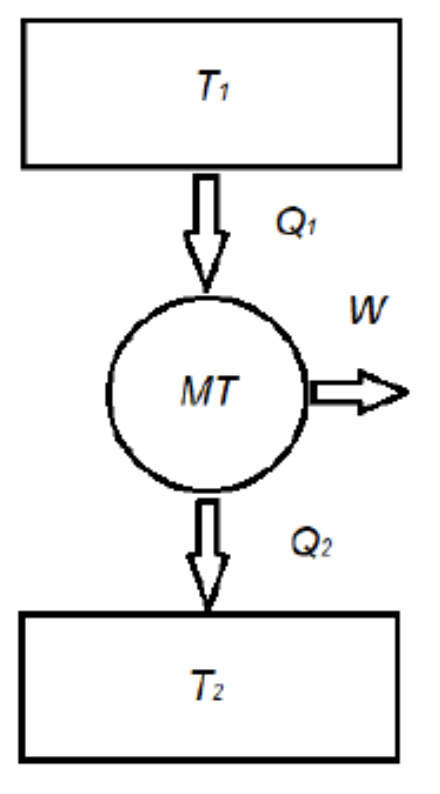
\includegraphics[width=0.3\linewidth, angle =90 ]{MT.png}
\end{center}

\section{Segundo principio}

\begin{gather*}
    \text{Máquina Térmica: } W = \left|Q_1\right|-\left|Q_2\right| \\ \eta_{MT}= \frac{W}{Q_1} = 1-\frac{Q_2}{Q_1}\Longrightarrow 1-\frac{T_2}{T_1}\\
    \text{Máquina Frigorífica}: Q_1 = Q_2 + W \quad \beta_{MF}=\frac{Q_2}{W} \\
    \beta_{BC}=\frac{Q_1}{W}=\frac{Q_2+W}{W}
\end{gather*}



\begin{gather*}
  \text{Entropía: } dS = \frac{\delta Q_\text{rev}}{T}\quad dS_{\text{Real}}\geq 0 \quad dS = \frac{\delta Q }{T}+dS_{\text{gen}}\\
  ds = \frac{du}{T} + \frac{Pdv}{T} = \frac{dh}{T}-\frac{vdP}{T}\\
  \text{Líquidos/Sólidos incompresibles: } c_V=c_P=C, dv=0\\
  ds = \frac{CdT}{T}\\
  \text{Gases ideales: } ds = \frac{c_V dT}{T} + \frac{Rdv}{v} = \frac{c_P dT}{T} -\frac{RdP}{P}
\end{gather*}
\subsection{Sistemas abiertos con j entradas y salidas y k fuentes de temperatura constante:}
\begin{gather*}
  dS_{VC}\geq \sum_j \delta m_j + \sum_k \frac{\delta Q_k}{T_k}\\
  \text{Escrito por unidad de tiempo en régimen estacionario:}\\
  -\sum_j s_j \dot{m}_j = \sum_k\frac{\dot{Q}_k}{T_k}+\dot{S}_\text{gen}\\
  \text{Trabajo para una máquina en flujo estable:}\\
  w_\text{rev}=-\int_{1}^{2}vdP - \Delta k_E - \Delta p_E
\end{gather*}

\subsection{Eficiencias isoentrópicas}

\begin{gather*}
  \eta^S_{\text{Bomba}}=\frac{W_\text{Rev}}{W_\text{Real}}= \frac{v\Delta P }{c\Delta T+v\Delta P }\\
  \eta^S_\text{Compresor}=\frac{W_\text{Rev}}{W_\text{Real}}=\frac{h_\text{out}^s-h_\text{in}}{h_\text{out}-h_\text{in}}\\
  \text{Gases Ideales Perf.}: \eta^S_\text{Compresor}=\frac{T_\text{out}^S-T_\text{in}}{T_\text{out}-T_\text{in}}\\
  \eta^S_{\text{Tobera}}=\left(\frac{c_\text{out}}{c_\text{out}^S}\right)^2 = \frac{h_\text{out}^+-h_\text{out}}{h_\text{out}^+-h_\text{out}^S}\\
  \eta^S_\text{Turbina}: \frac{W_\text{Rev}}{W_\text{Real}}=\frac{h_\text{in}-h_\text{out}^s}{h_\text{in}-h_\text{out}}\\
  \text{Gases Ideales Perf.}: \eta^S_\text{Turbina}=\frac{T_\text{in}^S-T_\text{out}}{T_\text{in}-T_\text{out}}
\end{gather*}

Donde $(\cdot)_\text{out}^S$ se obtiene mediante las relaciones de Poisson (considerando procesos isoentrópicos).

\section{Exergía}

\begin{gather*}
  \text{Exergía: } X=m\Phi= E-E_0 - T_0 (S-S_0) + P_0(V-V_0) = -W_\text{ú,máx}\\ %m(\Phi_1-\Phi_0) =
  W_\text{útil}= W-W_{\text{ATM}}= W - P_0(V-V_0)\\
  \text{Flow Exergy: } \Psi = (h-h_0)-T_0(s-s_0)+\frac{s^2}{2} +gz\\
    \text{Sistema A que intercambia calor con k fuentes a $T_K$:}\\
    \text{(visto desde cada fuente)}\\
  \Delta \Phi = \Delta EX = \Delta E_A - T_0 \Delta S_A + P_0 \Delta V_A + \sum_{k} Q_k(1 - \frac{T_0}{T_k})\\
\text{Irreversibilidad (visto desde el sistema):} \\
  I = T_0 S_{gen}
= T_0 \left( \Delta S_A - \sum_k \frac{Q_k}{T_k} \right)\\
  \text{Sistema dinámico:}\\
  \sum\left(1-\frac{T_0}{T_k}\right)\delta Q_k - [W-P_0  dV] +\\ \sum\delta m_i\Psi_i- \delta m_e\Psi_e-X_\text{destr}=dX
\end{gather*}

\section{Potencial químico}

\begin{gather*}
  dU = TdS - PdV + \sum_j \mu_j dn_j \qquad \mu_j = \frac{\partial U}{\partial n_j}\biggr\rvert_{S,V,n_k\neq n_j}\\
  dH = TdS + VdP + \sum_j \mu_j dn_j \qquad \mu_j = \frac{\partial H}{\partial n_j}\biggr\rvert_{S,P,n_k\neq n_j}\\
  \text{Energía libre de Helmholtz: } F= U-TS\\
  dF = -SdT + PdV + \sum_j \mu_j dn_j \qquad \mu_j = \frac{\partial F}{\partial n_j}\biggr\rvert_{T,V,n_k\neq n_j}\\
  \text{Energía libre de Gibbs: } H-TS\\
  dG = -SdT + VdP + \sum_j \mu_j dn_j \qquad \mu_j = \frac{\partial G}{\partial n_j}\biggr\rvert_{T,P,n_k\neq n_j}\\
  \text{Ecuación de Gibbs-Duhem: }\\
  SdT- VdP + \sum_j n_j d\mu_j=0
\end{gather*}
\begin{gather*}
  \mu = g = h-Ts, \quad h-h_0 = \int_{T_0}^{T}c_P(T)dT\\
  s-s_0 = \int_{T}^{T_0}\frac{c_P(T)}{T}dT - R\int_{P}^{P_0}\frac{dP}{P}\\
  \mu = \mu (T,P) = \varphi(T) + RT\ln(\frac{P}{P_0})\\
  \text{Condición de equilibrio de mezcla: } d\mu_j=d\mu_k
\end{gather*}

\begin{gather*}
  \text{Ley de Dalton: } P_j = \frac{n_j}{V}RT = y_j P_T, \quad y_j = \frac{n_j}{n_T} \quad ()_T = [N]_\text{Total}
\end{gather*}

\subsection{Entropía de mezcla}
\begin{gather*}
  \Delta S = n \sum_j y_j \Delta s_j\\
  \text{Gases ideales: }\Delta s_j = c_{Pj}\ln(\frac{T_2}{T_1})-R\ln(\frac{y_{j,2}P_2}{y_{j,1}P_1}),\\
  \text{Donde $T_k$ y $P_k$ son las temperaturas y presiones de cada estado}\\
  \text{y cantidad de gas ideal.}
\end{gather*}





% \lipsum[1-3]


\clearpage



\end{multicols}



\end{document}









